%%%%%%%%%%%%%%%%%%%%%%%%%%%%%%%%%%%%%%%%%%%%%%%%%%%%%%%%%%%%%%%%%%%%%%%%%%%
% Copyright (c) 2010 committers of YAKINDU and others.
% All rights reserved. This program and the accompanying materials
% are made available under the terms of the Eclipse Public License v1.0
% which accompanies this distribution, and is available at
% http://www.eclipse.org/legal/epl-v10.html
%
% Contributors:
%     committers of YAKINDU - initial API and implementation
%%%%%%%%%%%%%%%%%%%%%%%%%%%%%%%%%%%%%%%%%%%%%%%%%%%%%%%%%%%%%%%%%%%%%%%%%%%
\section{Detailed usage information}

\subsection{Regions}
\label{sec:Regions}

A region is a sub-state machine that runs concurrently to the other regions. To
serialize the processing of the sub-state machines within the regions, the
regions possess a priority. The region with the highest priority is processed
first.

\begin{figure}[ht] \center
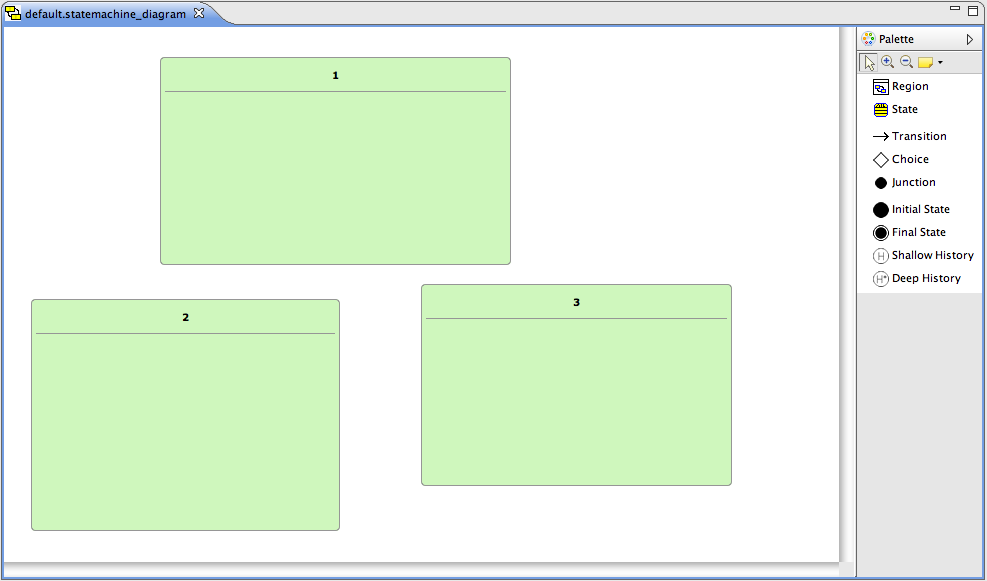
\includegraphics[width=0.7\textwidth]{./Pictures/RegionsPlain}
\caption{\label{fig:RegionsPlain}Three regions within a State Machine Diagram.}
\end{figure}

In the actual YAKINDU version, the regions are not hierarchically aggregatable.
  
\subsection{States}
\label{sec:States}

The states are the main elements of a state machine as they specify the possible
states the state machine consist of. Every state has a unique name, which must be
set by the user.

\begin{figure}[ht]
\center
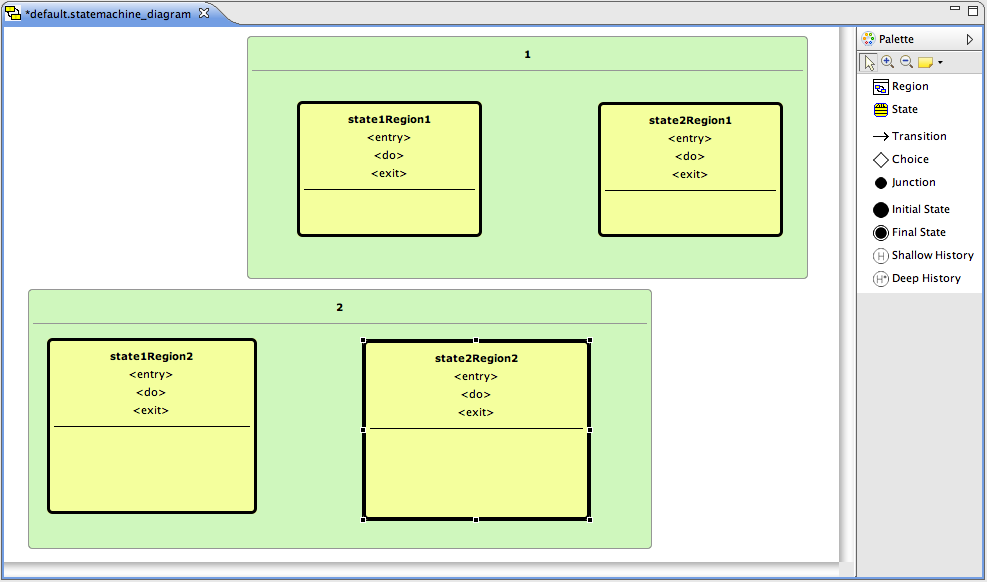
\includegraphics[width=0.7\textwidth]{./Pictures/statesInRegions}
\caption{\label{fig:statesInRegions}Two regions with two states each}
\end{figure}

The parameters of this state are:

\begin{itemize}
\item \textbf{Entry:} The actions, which are performed on the arrival in this
state are specified in the $<entry>$ area. 
\item \textbf{Do:} The actions, which are performed while the state does not 
change, is specified in the $<do>$ area.
\item \textbf{Exit:} The actions, which are performed when a status is left, is
specified in the $<exit>$ area.
\end{itemize}

%Hier fehlt noch: wie genau ist die "expression" die hier einzutragen ist definiert.
 
\newpage 

\subsection{Pseudostates}
\label{sec:Pseudostates}

Pseudostates are states, that do not have any $<entry>$, $<do>$ or $<exit>$
areas. These states are used to specify special states like the \textbf{Initial
State} or the \textbf{Final State}.

Actually the following states are defined:

\begin{itemize}
\item \textbf{Initial State:} The \textbf{Initial State} is the state where the
state machine or the sub-state machine specified by a region start with. Usually
the \textbf{Initial State} is connected unconditionally with another normal
state. 
\item \textbf{Final State:} The \textbf{Final State} is the state where a
state machine ends. When the \textbf{Final State} is reached, the state machine
usually stops processing. 
\item \textbf{Shallow History:} The \textbf{Shallow
History} carries the last active state within a sub-state machine. When this
sub-state machine is re-entered, the last active state is set active again. 
\item \textbf{Deep History:} The \textbf{Deep History} works as the \textbf{Shallow
History} but can also handle nested sub-state machines, so that the correct
nested sub-state machine is used when a sub-state machine is entered. 
\item \textbf{Choice:} A \textbf{Choice} a an element to branch a transition. Every
branch of a transition must have it's own transition condition. An example is a
transition, that is started with a trigger signal and then splits up to arrive at
state X or state Y depending on a guard variable. 
\item \textbf{Junction:} The
\textbf{Junction} connects two transitions that have the same target state.
\end{itemize}

\subsection{Transitions}
\label{sec:Transitions}

\textbf{Transitions} specify the change from one state to another. Every
\textbf{Transition} must have a condition on which the state switch takes place.
The syntax for this condition is:

\begin{verbatim}
Trigger1, Trigger2, \dots, TriggerN[Guard]/Action1; Action2; \dots ActionM; 
\end{verbatim}

\begin{itemize}
\item \textbf{Trigger:} A trigger is activated by an outside event. If more than
one trigger is specified all triggers are connected by \textbf{OR}.

A special trigger is specified by the \textit{after($<duration>$)} keyword. This
keyword defines a duration after which a transition is performed. The
$<duration>$ is an integer number with a specifier (e.g. $after(12s)$).

\item \textbf{Guard:}  A guard is a boolean expression. Example: \texttt{A==B}
\item \textbf{Action:} An action consists of instructions, that should be
performed during transition. This action should be short to have a reliable flow.
\end{itemize}

Additionally every \textbf{Transition} needs a unique priority. The reason is
that every \textbf{Transition} have to be unique, so that the state machine
always behalves in the same way independent of the sequence the
\textbf{Transitions} are created for example.

\subsection{Variables and Events}

The state machine is driven only by triggers and guarded variables, as discussed
in section \ref{sec:Transitions}. These two types of variable data can only be
used within a transition expression, if the variables and events (which results
in triggers) are defined.

To define a variable or an event, you open the \textbf{State Chart Interface} and
right-click on either \textbf{Events} or \textbf{Variables}.

The dialog \textbf{Create Variable} requests at least a name for the variable.
Additionally, the variable can have a \textbf{Port}. The \textbf{I/O-type}
specifies whether the variable is a local, input or output variable. At last, the
\textbf{Data Type} can be chosen between integer (int), floating point (double)
or boolean (bool).

Events are very similar to variables. The main difference during event creation
is that you can not specify a \textbf{Data Type} but a \textbf{Trigger Type}
which can hold the values \textit{raising}, \textit{falling} or \textit{either}.

\subsection{Interfaces}

To interact with the state machine the system designer can add interface
functions within an actions expression. These functions must follow the
\textbf{Action Function Pointer} definition (i.e. the function is returning void
and does not have any parameter). To meet the MISRA requirements, a function
pointer must be a constant pointer, which means that the interface function must
be bound to the state machine during compile time. So there is no late binding
available in this case.
